%!TEX root = ../../thesis.tex

\section{Proof and formalism}
\label{chapter:limitations:proof}

It is of paramount importance to understand the properties of our algorithm, and to be able to have some certitude about its convergence and accuracy properties. The work presented in this thesis neglected this aspect and relied only on empirical evaluation. The next step for a motivated person it to work on a formalism of our problem and to derive some usefull proof about some properties of the algorithm. In the following of this section we present a minimalist proof of the principle of our algorithm under extremely narrow condition.


\subsection{Assumptions}

It could be exemplified by an interface with two buttons, one for ``correct'' and one for ``incorrect'', but the mapping between the button and the meaning would not be defined in advance.

We further assume that the user is coherent and uses one signal for one meaning. The assumption is that the mapping between symbolic signals and their meaning can only be of two forms.

No errors from the teacher accorind to the optimal policies




\subsection{Illustration}


\begin{figure}[!ht]
\centering
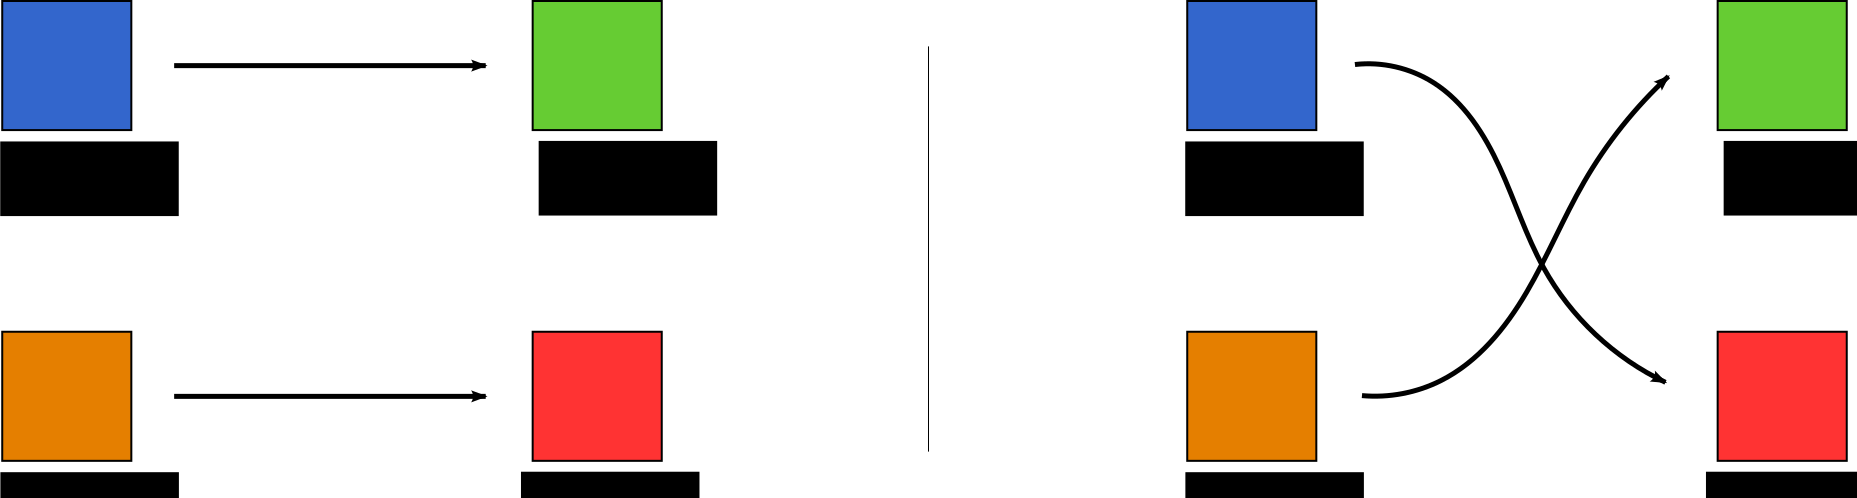
\includegraphics[width=\columnwidth]{\visualspdf/proof/mappings.pdf}
\caption{I}
\label{fig:proofmapping}
\end{figure} 


\begin{figure}[!ht]
\centering
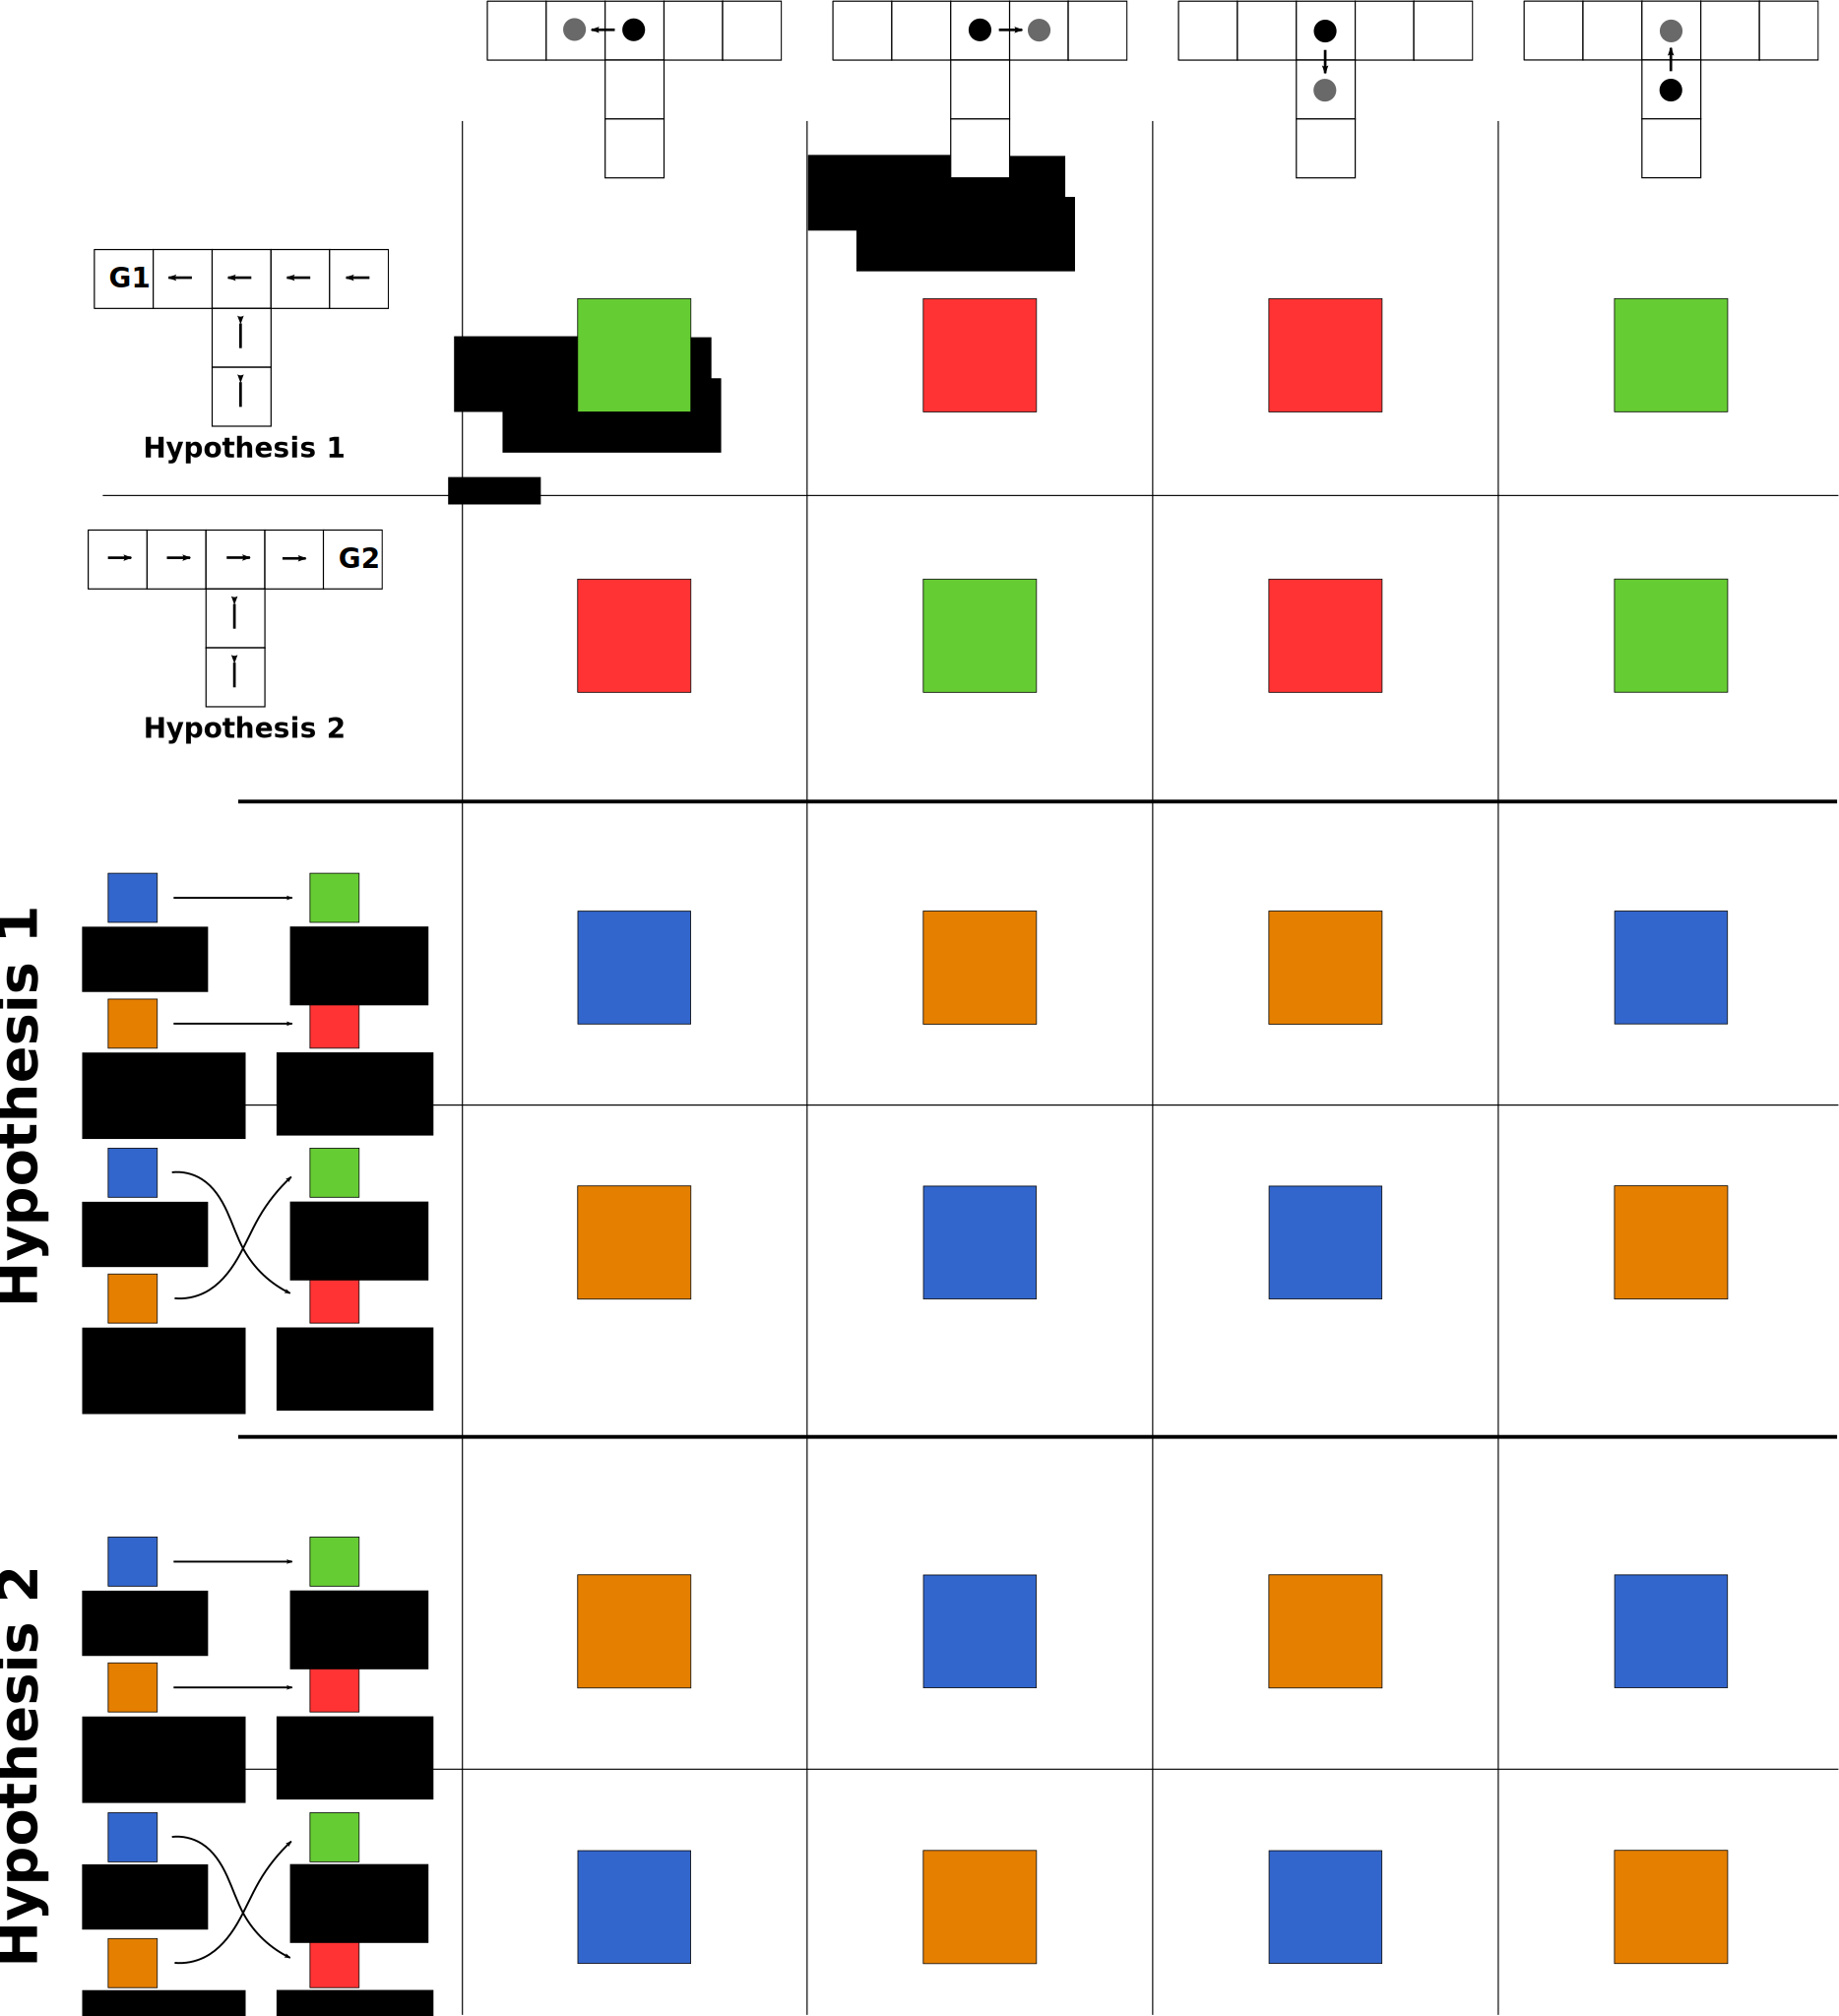
\includegraphics[width=\columnwidth]{\visualspdf/proof/symbolic_feedback.pdf}
\caption{I}
\label{fig:proofsymbolic}
\end{figure} 



\todo{figure with possible mapping}

For a particular hypothesis, the robot can assign hypothetic meanings)to the human signals knowing their are limited to a fixed set and according to the current state of the world. The machine is ``reasoning'' as follow: \emph{"If the human wants me to solve task G1 then when I performed action $a$ in state $a$ and he said ``oui'', he meant ``incorrect''"}. 

\todo{example step by step, first the world, one action, it interpretation wrt. each hypothesis, then accelerate and observe}

By creating a set of hypothesis, the system end-up with a set of possible interpretation of the human teaching signals. But as the user have only one objective in mind, here G1, only the correct interpretation will exhibit a coherence between the signals and their associated meanings. 

In our case, as the user is using symbolic signals, and that we assumed the user is coherent and use always the same symbol for the same meaning. We can infer that hypothesis G1 is the correct one as the resulting mapping between signal and meaning is more coherent.

\todo{For the symbolic case, and given specific constraint we will present a minimalist proof once the associated mathematical notation will be introduced}






\subsection{The proof}

Use the entropy information function to make this dummy proof.


performs once all state and action and collects the feedback


% \subsection{Discussion}

% The example described above simplifies the problem in many aspects. Indeed we assume the robot is already able to discriminate between perceptual events and has access to a unlabeled symbolic representation of the teaching signals. It would be the case when using a button based interface, however, when considering more ``natural'' means of interaction such as speech, the mapping between spoken words and their meaning should be learn by the machine. Indeed, the same word in never pronounced exactly the same way and some classification algorithm should be applied to train a discriminative model.